\documentclass[12pt]{report}

\usepackage{Dedman-Thesis-Latex-Template/sty/DL_thesis}  % Global Style for particular SMU College, e.g. DL_thesis.sty
\input{Dedman-Thesis-Latex-Template/latex/packages.tex}
% % Load additional packages here.
% Be careful of the loading order with respect to packages.tex as conflicts can easily arise.
% This is not a part of the base template and so will never be overwritten during updates.
\usepackage{tikz}
\usepackage{graphicx}
\usepackage{tikz-feynman}
\usepackage{fontspec}
%\usepackage{mathtools}
\newfontface\mathcursivefont{Daytonia.otf}
\DeclareTextFontCommand{\mathcurse}{\mathcursivefont}
 % Uncomment to load additional user required packages
\input{Dedman-Thesis-Latex-Template/latex/preamble.tex}
\input{Dedman-Thesis-Latex-Template/latex/custom_commands.tex}
% % Place your own personal commands here. 
% This is not a part of the base template and so will never be overwritten during updates.
 % Uncomment to use your own personal commands
\AuthorFirstName{Graduate}
\AuthorLastName{Student}
% \AuthorNameSuffix{Jr.}

% Title can be up to three lines of no more than 48 characters per line
% Write the title with the capitalization you want to be used in the abstract
\ThesisTitle{Smashy Physics:}{How I Pretended to Do More Smashing}{Using Smashy Math}
\GraduateDepartment{Physics}

\FirstDegree%
\FirstDegreeType{B.S.}
\FirstDegreeMajor{Physics}
\FirstDegreeUniversity{Undergraduate University}

\SecondDegree%
\SecondDegreeType{M.S.}
\SecondDegreeMajor{Physics}
\SecondDegreeUniversity{Southern Methodist University}

\ThesisDefenseDateYear{2022}
\ThesisDefenseDateMonth{April}
\ThesisDefenseDateDay{1}

\GraduationDateYear{2022}
\GraduationDateMonth{July}
\GraduationDateDay{1}

\SMUCollege{Dedman College}

% Committee
\AdvisorFullName{Dr.~Stephen Sekula}
\AdvisorTitle{Associate Professor}

\CommitteeMemberA{Dr.~Roberto Vega}
\CommitteeMemberTitleA{Professor}

\CommitteeMemberB{Dr.~Jingbo Ye}
\CommitteeMemberTitleB{Associate Professor}

\CommitteeMemberC{Dr.~External Member}
\CommitteeMemberTitleC{Assistant Professor}

\hypersetup{
 % Added more precise definition and options for Hyperref package.
 % Comment out or change hyperref preferences
 % \hypersetup should be loaded last
 bookmarksopen=true, % True: Open bookmark tree
 bookmarksnumbered=true, % True: put section numbers in bookmarks
 breaklinks=true, % True: split the url over multiple lines
 %   draft=true, % True: do not do any hyper linking
 filecolor=magenta, % Color of file links
 citecolor=blue, % Color of links to bibliography
 colorlinks=true, % False: boxed links; true: colored links
 linkcolor=blue, % Color of internal links
 linktocpage=true, % True: Makes the page number of TOC the link vs the text
 %   pagebackref=true, % True: Links references back to referring page
 pdfnewwindow=true, % True: URL links in new window
 plainpages=false, % True: do page number anchors as plain Arabic
 pdffitwindow=false, % Window fit to page when opened
 pdfmenubar=true, % Show Acrobat menu
 pdfstartview={FitH}, % Fits the width of the page to the window
 pdftoolbar=true, % Show Acrobat toolbar
 pdfauthor={Author}, % Author in PDF document properties
 pdfcreator={Author}, % Creator of the document in PDF document properties
 pdfkeywords={Keyword1} {Keyword2} {Keyword3} {Keyword4} {Author}, % List of keywords in PDF document properties
 pdfproducer={Producer}, % Producer of the document in PDF document properties
 pdfsubject={Subject}, % Subject of the document in PDF document properties
 pdftitle={Title of Dissertation}, % Title in PDF document properties
 unicode=false, % Non-Latin characters in Acrobat bookmarks
 urlcolor=cyan % Color of external links
}


\makeglossaries
\newglossaryentry{LHC}{
 text=LHC,
 long=Large Hadron Collider,
 name={\glsentrylong{LHC} (\glsentrytext{LHC})},
 first={\glsentryname{LHC}},
 sort={large hadron collider},
 description={Large Hadron Collider}
}

\newglossaryentry{thesis}{
 name=thesis,
 description={https://xkcd.com/1403/}
}


% \thesisdraft % uncomment if want draft printing

\begin{document}

\input{Dedman-Thesis-Latex-Template/latex/front_pages.tex}

\begin{thesis}

 \chapter*{Preface}\label{chapter:preface}
% c.f. https://tex.stackexchange.com/a/222961/152544
\addcontentsline{toc}{chapter}{\protect\numberline{}Preface}

The following is a summary of useful concepts in high energy particle physics.

\section{Units}\label{section:units}

Discussion of units

\section{Coordinates}\label{section:coordinates}

\gls{LHC} coordinate systems

\section{Statistics}\label{section:statistics}

Statistics in particle physics


 \chapter{Introduction}\label{chapter:introduction}

%The basic structure of every lab report you've ever done is: 
%    introduction,
%    theory,
%    experimental setup,
%    procedure,
%    results,
%    conclusion.
%
%This thesis is essentially following that same format:
%    Introduction,
%    Standard Model... and Signal modelling? (theory),
%    LHC and ATLAS and Trigger (experimental setup)
%    Reconstruction, Selection, Background Estimation (procedure)
%    results (...)
%    conclusion

The Higgs Boson was proposed as a fundamental particle in 1964,
    and has been a driving factor in particle physics research ever since.
Though it was jointly discovered in 2012 by the ATLAS and CMS collaborations,
    there are still a number of properties of the Higgs which have yet to be measured.
Chief among these are two of the Higgs' self-coupling constants, \kl and \kvv,
    which determine how strongly the Higgs interacts with both itself and with vector bosons.
This analysis performs a search for the rare,
    as-yet unseen diHiggs interaction in order to set tighter constraints on these coupling values.
The search utilizes the Vector Boson Fusion production mechanism of the diHiggs process,
    identifying the process in the 4b final state.
This is performed using 126 $\textit{fb}^{-1}$ of data from Run 2 of ATLAS.

This thesis will begin by first explaining the importance of the Higgs Boson to the field of particle physics,
    as well as the relevance of the aforementioned \kl and \kvv coupling constants.
I will then describe the physical effects of these constants,
    and how those effects can be exploited in order to make measurements of them.
These topics comprise Chapter \ref{chapter:theory}.
Following from the theoretical discussion, I will discus the experimental equipment and setup used to perform the  measurments.
The experimental setup is discussed across three chapters.
Chapter \ref{chapter:lhc} discusses the Large Hadron Collider, the machine which generates the conditions necessary to produce diHiggs process.
Actual observation of the process once generated is carried out by the ATLAS particle detector array and its Trigger system,
    described in Chapters \ref{chapter:atlas} and \ref{chapter:trigger}.
The reconstruction process, described in Chapter \ref{chapter:reconstruction},
    entails how data observed by ATLAS is analyzed in order to determine which physics processes occured during the myriad observed interactions.
Background processes are removed from the data set using a selection procedure explained in Chapter \ref{chapter:selection},
    and the contribution of the background events which remain is estimated using data-driven technique cataloged in Chapter \ref{chapter:background}. 
The background estimation process makes use of a neural network reweighting procedure, which I personally configured and ran the training for.
My primary contribution to the analysis however, comes in the form of the signal model that constitutes the hypothesis for the behaviour of the Higgs Boson.
The signal model makes use of a Monte-Carlo sample combination technique, which I developed and optimized in the context of the \vbfproc process.
This is elaborated upon in Chapter \ref{chapter:signal}.
Finally, in Chapter \ref{chapter:results}, this hypothesis alongside the background estimate are compared against the data observed from ATLAS,
    in order to make constraints on the diHiggs self-coupling constants.



%This is the first chapter of the \gls{thesis}.~\cite{Aaboud:2016mmw,Bruning:782076}

\section{Creating Figures}\label{sec:figures}
\begin{figure}[htpb]
 \centering
 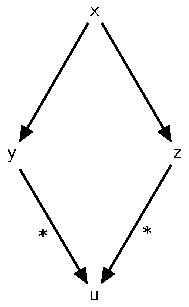
\includegraphics{introduction/example.pdf}
 \caption[Example placeholder figure with a citation~\cite{Higgs:1964ia} and shorter List of Figures caption.
  The List of Figures is protected from first use of glossary entries or acronyms like \acrlong{LHC}.]{%
  This is a placeholder figure to act as an example.
  Here we cite a new reference in the caption to demonstrate that given the package configuration our order of references will not be distributed by the table of contents~\cite{Higgs:1964ia}.}\label{fig:test_figure}
\end{figure}

As can be seen in \Cref{fig:subfigure_example}, the subfigures are independent of each other such that \Cref{fig:subfigure_1} and \Cref{fig:subfigure_2} can be accessed separately.

\begin{figure}[htbp]
 \centering
 \begin{subfigure}[t]{0.48\textwidth}
  \centering
  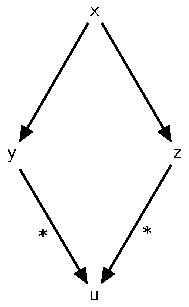
\includegraphics[width=0.3\textwidth]{introduction/example.pdf}
  \caption[Short List of Figures captions work with subfigures too.]{%
   This is the first figure of two, in this example, and its own independent subfigure.}
  \label{fig:subfigure_1}
 \end{subfigure}%
 \quad
 \begin{subfigure}[t]{0.48\textwidth}
  \centering
  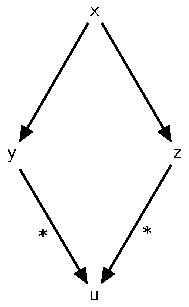
\includegraphics[width=0.3\textwidth]{introduction/example.pdf}
  \caption[Which makes the List of Figures readable and actually helpful.]{%
   As the \texttt{t} alignment option was chosen for the subfigures, they are still properly aligned vertically even though this caption is longer.}
  \label{fig:subfigure_2}
 \end{subfigure}
 \caption{An example of a figure that consists of two subfigures.}
 \label{fig:subfigure_example}
\end{figure}

As an example of an equation formatted in ``\href{https://www.overleaf.com/learn/latex/Display_style_in_math_mode}{display style}'' the equation for the fiducial cross section from~\cite{Aaboud:2016mmw} is reproduced as \Cref{eq:fiducial_cross_section}:
\begin{equation}
 \sigma_{\mathrm{inel}}^{\mathrm{fid}} \left(\zeta > 10^{-6}\right) = \frac{N - N_{\mathrm{BG}}}{\epsilon_{\mathrm{trig}} \times \mathcal{L}} \times \frac{1 - f_{\zeta < 10^{-6}}}{\epsilon_{\mathrm{sel}}}
 \label{eq:fiducial_cross_section}
\end{equation}

\section{Creating Tables}\label{sec:tables}

To create tables in \LaTeX{} it is highly recommended to use the \href{https://www.ctan.org/pkg/booktabs}{\texttt{booktabs}} package.
It allows for very elegant and clean table creation, such as \Cref{table:natural_units}.
If you want to create a table quickly, or have a CSV file that you'd like to quickly turn into a table there are various \href{https://www.tablesgenerator.com/}{online \LaTeX{} table generators}.

\begin{table}[htpb]
 \centering
 \caption[Common quantities in particle physics in natural and SI units.]{%
  Common quantities in particle physics given in both natural units and SI units.}
 \begin{tabular}{@{}llll@{}} \toprule
  Quantity         & Natural Units                 & Natural Units (dimensionful)            & SI Units                                              \\ \midrule
  Speed            & $1$                           & $c$                                     & $3.0\times 10^{8}~\mathrm{m}/\mathrm{s}$              \\
  Angular Momentum & $1$                           & $\hbar$                                 & $10^{34}~\mathrm{m}^2 \,\mathrm{kg}/\mathrm{s}$       \\
  Energy           & $\mathrm{GeV}$                & $\mathrm{GeV}$                          & $1.6\times 10^{-10}~\mathrm{J}$                       \\
  Momentum         & $\mathrm{GeV}$                & $\mathrm{GeV}/c$                        & $1\times 10^{-19}~\mathrm{kg}\,\mathrm{m}/\mathrm{s}$ \\
  Mass             & $\mathrm{GeV}$                & $\mathrm{GeV}/c^{2}$                    & $1.8\times 10^{-27}~\mathrm{kg}$                      \\
  Time             & $1/\mathrm{GeV}$              & $\hbar/\mathrm{GeV}$                    & $6.6\time 10^{-25}~\mathrm{s}$                        \\
  Length           & $1/\mathrm{GeV}$              & $\hbar c/\mathrm{GeV}$                  & $2\times 10^{-16}~\mathrm{m}$                         \\
  Electric Charge  & $1$                           & $e/\sqrt{4\pi \alpha_{\mathrm{em}}}$    & $5.3\times 10^{-19}~\mathrm{C}$                       \\
  Magnetic Field   & $\left(\mathrm{GeV}\right)^2$ & $\left(\mathrm{GeV}\right)^2/\hbar c^2$ & $5\times 10^{16}~\mathrm{T}$                          \\
  \bottomrule
 \end{tabular}\label{table:natural_units}%
\end{table}

Good table design requires some thought and work, so it may be worth a look through some examples:
\begin{itemize}
 \item \href{https://tex.stackexchange.com/questions/238503/tip-on-how-to-make-a-visually-good-table}{TeX StackExchange: Tip on how to make a visually good table}
 \item \href{https://twitter.com/edwardtufte/status/451820483109847040?lang=en}{Edward Tufte endorsed} example from \href{http://static1.squarespace.com/static/56713bf4dc5cb41142f28d1f/t/56fd4c83746fb9261146eed5/1459440776291/ClearOffTheTableMd.gif}{Darkhorse Analytics}
\end{itemize}

\section{Dealing with Widows and Orphans}\label{sec:widos_and_orphans}

To reduce the difficulty of dealing with widowed text (the last line of a paragraph at the start of a page) and orphaned text (the first line of paragraph at the end of a page) the \href{https://ctan.org/pkg/nowidow?lang=en}{\texttt{nowidow}} package is used.
However, that doesn't solve the issue of orphaned section titles.
The user must manually do this, but the following \href{https://texfaq.org/FAQ-widows}{simple advice from \TeX{} FAQ} is recommended:

\begin{quote}
 Once you've exhausted the automatic measures, and have a final draft you want to ``polish'', you should proceed to manual measures.
 To get rid of an orphan is simple: precede the paragraph with \texttt{\textbackslash clearpage} and the paragraph can’t start in the wrong place.
\end{quote}



 \chapter{Printer Calibration}\label{chapter:printer_calibration}

As you may know, printers do not print your PDF file exactly.
They will scale it to match their own preset configurations and potentially add padding spaces around the edges.
There is no way to control for this as every printer is unique and there are no base standards.
The only thing a user can do is have their generated PDF file have the correct distances and then ask that the person printing their document calibrate the printer accordingly.

\printercalibration{}

\vspace{2in}
This chapter will provide printer calibrations.
All the \textcolor{red}{red lines} drawn are $1$~inch in length.
All the \textcolor{blue}{blue lines} drawn are $2$~inches in length.
These are drawn from the edge of the document in TikZ, which has good distance metrics built into it, so these distances are accurate.
Print this page and measure the margins and the length of the arrows.
If your measurements do not match those printed \textbf{you need to calibrate your printer}.
It is probable that your printer has an option that is along the lines of ``actual size'', so that might be a good starting point.
It can also help to turn on \verb|\geometry{showframe=true}| in your preamble.


 \StartAppendix%

 \chapter{An Appendix}\label{appendix:ATLAS_detector}

Appendix text goes here.


 % Glossary
 % Check with specific department on the style to use
 \clearpage
 \singlespacing%
 \setglossarystyle{list}
 \printglossary[title=GLOSSARY,toctitle=GLOSSARY]
 \doublespacing%

 % Bibliography goes below
 % Check with specific department on the appropriate
 % bibliography style to use

 \nocite{*}
 \bibliographystyle{bib/JHEP}
 \raggedright
 \bibliography{bib/theory}

\end{thesis}
\end{document}
